\chapter{Deployment and Testing}
\label{ch:deployment-and-testing}
aiVLE 2.0, especially aiVLE Worker and aiVLE Grader, is designed to be highly scalable and easy to deploy. However, just like any distributed systems, being able to run the individual components on a single machine is one thing, having all the components cooperate on separate machines to achieve actual distribution is another. Thus, to pave way for production deployment in the next academic year, and to demonstrate the actual performance of such a distributed system, we performed a complete deployment using several SoC cluster nodes and did several experiments/benchmarks on the system.

There are three sections covering both the deployment and tests this chapter: Section~\ref{s:deployment} describes the deployment environment, deployment steps and issues we encountered before making the system fully functional on SoC compute cluster. Section~\ref{s:load-balance-exp} discusses the experiment of load balancing among \textbf{multiple} worker nodes. Section~\ref{s:concurrency-exp} discusses the experiment of running evaluation jobs concurrently on a \textbf{single} worker node.

\section{Deployment}
\label{s:deployment}
Note that this deployment happened during the winter break (November 2021 to January 2022). Therefore some later updates to the aiVLE Web and Worker are not included during this deployment (most notably, resource-sensitive load balancing as mentioned in Section~\ref{ss:aivle-worker-resource-awareness} and Section~\ref{ss:aivle-web-load-balancing}). However, this does not affect the test results as the experiments are designed to have no system overloading (see Section \ref{sss:choice-of-params}).

In specific, the exact versions used are (tag with GitHub link):
\begin{itemize}
    \item aiVLE Web: deploy-1 (\href{https://github.com/edu-ai/aivle-web/releases/tag/deploy-1}{https://github.com/edu-ai/aivle-web/releases/tag/deploy-1})
    \item aiVLE Worker: v0.1.2 (\href{https://github.com/edu-ai/aivle-worker/releases/tag/v0.1.2}{https://github.com/edu-ai/aivle-worker/releases/tag/v0.1.2})
\end{itemize}

\subsection{Environment}
\label{ss:deployment-environment}
aiVLE Worker is deployed on SoC compute cluster \texttt{xgpg0, xgpg1, xgpg2} with the following configuration:
\begin{itemize}
    \item Operating System (Code~\ref{code:deployment-os}): Ubuntu 20.04 LTS with Linux kernel version 5.4.0
    \item GPU (Code~\ref{code:deployment-gpu}): NVIDIA A100-PCI, Driver 495.29, CUDA 11.5
    \item CPU: 2x AMD Epyc 7352, in total 48 cores/96 threads, base clock 2.3GHz
    \item RAM: 256GiB DDR4
\end{itemize}

\begin{code}
\begin{minted}[frame=lines,framesep=2mm,baselinestretch=1.2,bgcolor=LightGray,fontsize=\footnotesize,linenos,samepage]{shell}
> cat /proc/version
Linux version 5.4.0-91-generic (buildd@lcy01-amd64-017) 
(gcc version 9.3.0 (Ubuntu 9.3.0-17ubuntu1~20.04)) #102-Ubuntu SMP Fri Nov 5 16:31:28 UTC 2021
\end{minted}
\captionof{listing}{Deployment Environment - Operating System}
\label{code:deployment-os}
\end{code}

\begin{code}
\begin{minted}[frame=lines,framesep=2mm,baselinestretch=1.2,bgcolor=LightGray,fontsize=\footnotesize,linenos,samepage]{shell}
> nvidia-smi
+-----------------------------------------------------------------------------+
| NVIDIA-SMI 495.29.05    Driver Version: 495.29.05    CUDA Version: 11.5     |
|-------------------------------+----------------------+----------------------+
| GPU  Name        Persistence-M| Bus-Id        Disp.A | Volatile Uncorr. ECC |
| Fan  Temp  Perf  Pwr:Usage/Cap|         Memory-Usage | GPU-Util  Compute M. |
|                               |                      |               MIG M. |
|===============================+======================+======================|
|   0  NVIDIA A100-PCI...  On   | 00000000:01:00.0 Off |                    0 |
| N/A   49C    P0    36W / 250W |      0MiB / 40536MiB |      0%      Default |
|                               |                      |             Disabled |
+-------------------------------+----------------------+----------------------+
\end{minted}
\captionof{listing}{Deployment Environment - GPU}
\label{code:deployment-gpu}
\end{code}

aiVLE Web is deployed on a \href{https://linode.com/}{Linode} Nanode 1GB VPS (virtual private server) with 1 virtual CPU core and 1 GiB of RAM. We carefully picked the parameters to avoid the aiVLE Web server being the bottleneck of all experiments (see Section~\ref{sss:choice-of-params}).

\subsection{Limitations}
\label{ss:deployment-limitations}
As with every distributed system, even if the system works on a few machines, it does not necessarily mean the system will work or scale well to dozens or even hundreds of machines. While we design the system to be highly scalable, and the underlying technologies (i.e., Celery as Python library and RabbitMQ as message queue broker) have proven to be effective on hundreds of machines, we are never certain until we actually scale the system to that many nodes and put it under pressure.

Unfortunately, for the time being, we are unable to materialize such a large-scale experiment: as we could only secure access to three machines in the SoC compute cluster. Also, at the moment, the tasks were not demanding enough to put the system at such a scale under considerable pressure. For example, on the \texttt{xgpg*} nodes used for this experiment, every evaluation takes $\sim$10 seconds to finish, which is too short for even tens of worker nodes. For the evaluation subsystem to be stressed, we at least need to keep the task queue ``filled''. In other words, the rate of submitting new jobs into the task queue should be comparable to the rate of workers finishing jobs. However, with each job only taking $\sim$10 seconds, suppose we have 50 workers, our rate of consumption would be $50/10=5$ jobs per second (every 10 seconds we can process 50 jobs). If we assume each submission to be $\sim$20MiB\footnote{Many deep learning models are much larger, so we are having a relatively conservative estimation here}, it would require at least 100MiB per second of network throughput, which is already approaching the limit of gigabit Ethernet available on most machines.

Therefore, with our current resources and setup, we could not properly evaluate the scalability potential of aiVLE 2.0. However, our experiment setup is on par with the resources available to the CS4246 teaching team, and aiVLE 2.0 is shown to have a much higher utilization rate of computational power. As a result, aiVLE 2.0 can process submissions with much smaller delays. In addition, properties like fair distribution and small worker overhead remain stable regardless of the number of nodes, so they DID get properly evaluated in our experiments.

In short, we are cautiously optimistic about the scalability of aiVLE 2.0 as we do not yet have experiment data to support it, but we are confident that it can support CS4246 teaching much more effectively from the results.

\subsection{Steps}
To simulate the production deployment process, we started everything afresh. The following steps are sufficient for any deployment from the ground up:

\begin{enumerate}
    \item Prepare the message queue broker: either by installing \href{https://www.rabbitmq.com/}{RabbitMQ} or using cloud message queue provider such as \href{https://www.cloudamqp.com/}{CloudAMQP}. In our case, we installed RabbitMQ on the same VPS with aiVLE Web.
    \item Install and start aiVLE Web on the master server.  The aiVLE Web Read-me\footnote{\href{https://github.com/edu-ai/aivle-web\#readme}{https://github.com/edu-ai/aivle-web\#readme}} is the definitive guide on this process.
    \item Setup the users, courses, tasks in aiVLE Web via its RESTful API or Django admin panel.
    \item Prepare the worker nodes with necessary dependencies (i.e., Firejail, Pip, Virtualenv, CUDA drivers). In our case, we requested the cluster admins to install Firejail as all other dependencies are already available.
    \item Install and start aiVLE Worker on the worker nodes. aiVLE Worker Read-me\footnote{\href{https://github.com/edu-ai/aivle-worker\#readme}{https://github.com/edu-ai/aivle-worker\#readme}} describes this process in detail.
\end{enumerate}

There are some issues we found during the deployment process. None of which is critical in a sense that we eventually found workarounds without modifying any existing codebase or design. You may find the details in Appendix~\ref{appendix:deployment-issues}.

\section{Load Balance Experiment}
\label{s:load-balance-exp}
In this section, we will discuss the experiments about load balancing evaluation jobs among \textbf{multiple} worker nodes. There are three objectives for this series of experiments:

\begin{enumerate}
    \item Show that the evaluation system scales well horizontally to several worker nodes.
    \item Show that the tasks are distributed evenly among worker nodes.
    \item Show that the worker nodes are fully utilized during stressful load.
\end{enumerate}

Raw logs and analyzing scripts can be found in \href{https://github.com/edu-ai/aivle-experiment-logs}{aiVLE experiment logs repository}\footnote{\href{https://github.com/edu-ai/aivle-experiment-logs}{https://github.com/edu-ai/aivle-experiment-logs}}. Correspondence between experiment setup and log file index is shown in Table~\ref{tab:load-balance-exp}.

\begin{table}[H]
\centering
\begin{tabular}{|c|c|c|c|c|c|}
\hline
\multicolumn{1}{|l|}{\begin{tabular}[c]{@{}l@{}}Web\\ log index\end{tabular}} & \multicolumn{1}{l|}{\begin{tabular}[c]{@{}l@{}}Worker\\ log index\end{tabular}} & \multicolumn{1}{l|}{Node count} & \multicolumn{1}{l|}{\begin{tabular}[c]{@{}l@{}}Concurrency \\ of worker\end{tabular}} & \multicolumn{1}{l|}{Submission count} & \multicolumn{1}{l|}{\begin{tabular}[c]{@{}l@{}}Concurrency \\ of submission\end{tabular}} \\ \hline
5 & 2 & 3 & 8 & 100 & 100 \\ \hline
6 & 3 & 2 & 8 & 100 & 100 \\ \hline
7 & 4 & 1 & 8 & 100 & 100 \\ \hline
\end{tabular}
\caption{Load Balancing Experiment Setup}
\label{tab:load-balance-exp}
\end{table}

\subsection{Methodology}
\label{ss:lb-exp-meth}
Since the evaluation task and all worker nodes are exactly the same, we have four parameters/variables to adjust:
\begin{enumerate}
    \item Node count: number of active nodes during the experiment.
    \item Concurrency of worker: maximum number of concurrent evaluation jobs allowed on \emph{each} worker node.
    \item Submission count: number of evaluation jobs submitted to the task queue.
    \item Concurrency of submission: maximum number of threads submitting jobs concurrently. Note that if this number is comparable to the submission count, master server will be blocked until all submissions are accepted (i.e., it will not distribute evaluation jobs to any of the worker nodes until all submissions are well-received)\footnote{This is because the submission rate is significantly larger than how fast the master server can process requests, and these submissions will pile up in the requests queue. Since the master server processes requests on a first-come, first-served basis, it is effectively blocked before all submissions are accepted. Of course this number cannot grow indefinitely as any machine will eventually run out of available threads or network bandwidth. Consequently, the submission count cannot grow indefinitely either as it should be comparable to the concurrency of submission. Section~\ref{sss:choice-of-params} will discuss the preliminary experiments that aim to find these upper bounds.\label{fn:concurrency-of-submission}}.
\end{enumerate}

In this section and Section~\ref{s:concurrency-exp}, submission count and concurrency of submission are both 100. This means before the first job is assigned to any of the worker nodes, 100 jobs are already queued. This is to ensure there will always be sufficient tasks for the workers to work on - if concurrency of submission is significantly smaller than the number of submissions, then the rate of submitting job may dictate the rate of workers finishing jobs, which is undesirable for our stress-oriented experiments.

For load balance experiment, we \textbf{fix concurrency on all workers to be 8}, measure \textbf{time taken} to finish 100 submissions with
\begin{itemize}
    \item 1 node (\texttt{xgpg0})
    \item 2 nodes (\texttt{xgpg0,1})
    \item 3 nodes (\texttt{xgpg0,1,2})
\end{itemize}

On the master server (aiVLE Web), we logged the critical phases of each submission with a timestamp, in specific, there is a timestamped record when
\begin{enumerate}
    \item submission is received
    \item evaluation job is submitted to task queue
    \item evaluation job is picked up by a worker
    \item evaluation job is being worked on by a worker
    \item evaluation job is terminated (either finished or failed)
\end{enumerate}

The start time is defined to be the earlier of 1) the latest ``submission is received'' record or 2) the earliest ``evaluation job is picked up by a worker'' record. The finish time is defined to be the latest ``evaluation job is terminated'' record. The total time is defined to be the difference between the finish time and the start time. The detailed method of calculating time taken to finish all submissions can be found in the \href{https://github.com/edu-ai/aivle-experiment-logs/blob/main/web/analyze.ipynb}{analyze script}. Note that the focus of this experiment is on the \textbf{evaluation (sub)system}, not the entire system. For example, before we can start evaluation jobs, we need to upload the student submission first. However, the submission itself could take a significant amount of time depending on the server workload. Such preparation time is an irrelevant variable and should be excluded from our calculation. The definition of the start time here, combined with our effort to adjust the parameters such that evaluation starts only after all submissions are received, achieved such exclusion.

On each worker node, we also logged the timestamped GPU utilization rate and VRAM usage periodically (Figure~\ref{fig:experiment-lb-utilization-plot}). This helps us understand whether all worker nodes are busy most of the time - unnecessary idling is a sign of poor load balancing.

\begin{figure}[H]
    \centering
    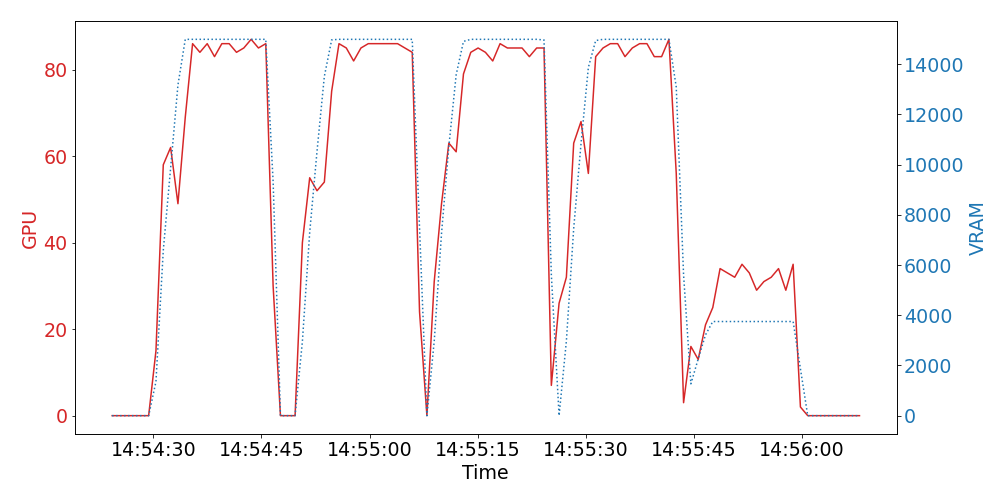
\includegraphics[width=\textwidth]{images/worker-utilization.png}
    \caption{GPU/VRAM Utilization Plot from \texttt{xgpg0\_2.log}}
    \label{fig:experiment-lb-utilization-plot}
\end{figure}

\subsubsection{Choice of Parameters}
\label{sss:choice-of-params}

There are two parameters that remain unexplained: number of total submissions (100) and maximum concurrent evaluations on each worker (8).

For the maximum concurrency allowed on each worker, we want the concurrency to be as large as possible (so that we properly ``stress'' the system) without overwhelming the system (so that the scaling overhead is mostly because of our task queue system instead of overwhelmed worker nodes). Since our evaluation task is mostly GPU-bounded, we performed experiments on a single machine with concurrent evaluation ranging from 2 to 16 and observed both the \textbf{GPU} utilization and \textbf{VRAM} utilization. With 40GiB of VRAM, we cannot overload the VRAM with even 16 concurrent jobs as each job takes less than 2GiB of VRAM. On the other hand, GPU utilization increases linearly with number of concurrent jobs until more than 8 jobs. Increasing more jobs will not significantly increase the GPU utilization after 8 jobs, indicating that the machine could only handle up to 8 jobs without significantly degraded per-job performance.

For the total submission count, it is bounded by the maximum concurrent submission our server and network can handle (see Footnote~\ref{fn:concurrency-of-submission}). We performed preliminary experiments with 1500 (\href{https://github.com/edu-ai/aivle-experiment-logs/blob/main/web/debug.log.1}{\texttt{debug.log.1}}) and 250 (\href{https://github.com/edu-ai/aivle-experiment-logs/blob/main/web/debug.log.4}{\texttt{debug.log.4}}) total submissions, and found the submission client could not reach sufficient request concurrency (i.e., large enough such that no evaluation will happen before all submissions are received) in both cases. In fact, for \texttt{debug.log.1} and \texttt{debug.log.4}, the average time taken to finish evaluating one submission is $\sim$25 seconds, and we did observe evaluation jobs started before submissions are concluded. Given that the optimal time (i.e., time taken without any communication overhead) is $\sim$15 seconds, this confirms our intuition that not queuing up all submissions before starting evaluation severely hurts the accuracy of these experiments. On the contrary, for scenarios listed in Table~\ref{tab:load-balance-exp}, the average time is $\sim$18 seconds, which is much closer to the optimal time, and $\sim$3 seconds of overhead seems acceptable considering it needs to download and decompress the student submission first.

\subsection{Results}
\label{ss:load-balancing-exp-results}

First, for the performance of load balancing, below are the times for each test case:

\begin{itemize}
    \item 1 node: 235.426s (baseline)
    \item 2 nodes: 128.261s (91.78\%)
    \item 3 nodes: 92.475s (84.86\%)
\end{itemize}
The percentage is the scaling efficiency defined by $\frac{\text{Optional time}}{\text{Measured time}}\times 100\%$ where \emph{Optimal Time} is defined as (taking $N$ as the number of nodes, $t_0$ as the time taken with one node) $\frac{t_0}{N}$. We have observed satisfactory scaling efficiency in both 2-node and 3-node configurations.

Second, for the fairness of load balancing, below are the numbers of jobs assigned to each worker node (when there are more than one node):

\begin{itemize}
    \item 2 nodes: \texttt{\{celery@xgpg0: 50, celery@xgpg1: 50\}}
    \item 3 nodes: \texttt{\{celery@xgpg0: 34, celery@xgpg1: 36, 'celery@xgpg2': 30\}}
\end{itemize}
The jobs are nearly equally distributed in both cases, meaning that our round-robin load balancing mechanism is working as expected.

Third, for the utilization of system resources, since our task is GPU-bound, Figure~\ref{fig:experiment-lb-utilization-plot} plots the GPU and VRAM utilization for one of the worker nodes (others are similar). We have observed stable GPU utilization of $\sim 85\%$ at peak, and a busy rate of $\sim 96\%$, meaning we have very good utilization of worker node resources.

\begin{figure}[H]
    \centering
    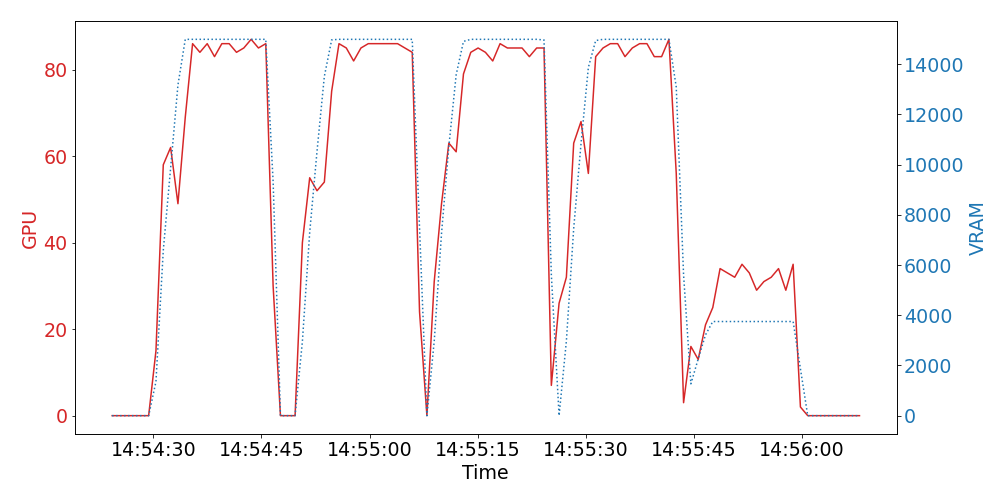
\includegraphics[width=\textwidth]{images/worker-utilization.png}
    \repeatcaption{fig:experiment-lb-utilization-plot}{GPU/VRAM Utilization Plot from \texttt{xgpg0\_2.log}}
\end{figure}

\section{Concurrency Experiment}
\label{s:concurrency-exp}
In this section, we will discuss the experiments about running multiple evaluation jobs \textbf{concurrently} on a \textbf{single} worker node. The objective is to show that our worker node can process multiple submissions in parallel with linear scalability.

Raw logs and analyzing scripts can be found in \href{https://github.com/edu-ai/aivle-experiment-logs}{aiVLE experiment logs repository}. For correspondence between experiment setup and log file index, please refer to Table~\ref{tab:concurrency-exp}.

\begin{table}[H]
\centering
\begin{tabular}{|c|c|c|c|c|c|}
\hline
\multicolumn{1}{|l|}{\begin{tabular}[c]{@{}l@{}}Web\\ log index\end{tabular}} & \multicolumn{1}{l|}{\begin{tabular}[c]{@{}l@{}}Worker\\ log index\end{tabular}} & \multicolumn{1}{l|}{Node count} & \multicolumn{1}{l|}{\begin{tabular}[c]{@{}l@{}}Concurrency \\ of worker\end{tabular}} & \multicolumn{1}{l|}{Submission count} & \multicolumn{1}{l|}{\begin{tabular}[c]{@{}l@{}}Concurrency \\ of submission\end{tabular}} \\ \hline
7 & 4 & 1 & 8 & 100 & 100 \\ \hline
8 & 5 & 1 & 4 & 100 & 100 \\ \hline
9 & 6 & 1 & 2 & 100 & 100 \\ \hline
10 & 7 & 1 & 1 & 100 & 100 \\ \hline
\end{tabular}
\caption{Per-worker Concurrency Experiment Setup}
\label{tab:concurrency-exp}
\end{table}

\subsection{Methodology}
For explanation of parameters/variables, and the method of measuring total time please refer to Section~\ref{ss:lb-exp-meth}. For the per-worker concurrency experiment, we activate \textbf{only one} worker node, and measure \textbf{time taken} to finish 100 submissions with the \textbf{concurrency of worker} ranging from 1, 2, 4 and 8.

\subsection{Results}

\begin{itemize}
    \item concurrency = 1: 1558.811s (baseline)
    \item concurrency = 2: 859.237s (90.71\%)
    \item concurrency = 4: 422.744s (92.18\%)
    \item concurrency = 8: 235.426s (82.77\%)
\end{itemize}

Similar to the first part of Section \ref{ss:load-balancing-exp-results}, the percentage in the end is the scaling efficiency. Its definition is also similar by changing the meaning of $N$ to the concurrency number. We have achieved over 90\% efficiency when the system is not too heavy-loaded, and over 80\% efficiency when the system is at its absolute limit. We are satisfied with such per-instance concurrency performance.
